\documentclass{minimal}
\usepackage{tikz}
\usepackage[T1]{fontenc}
\usepackage[default]{gillius}

\usetikzlibrary{positioning}
\usetikzlibrary{calc}
\usetikzlibrary{arrows}
\usetikzlibrary{automata}

\begin{document}

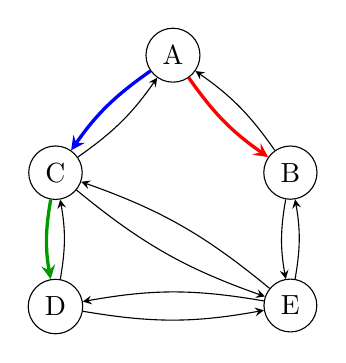
\begin{tikzpicture}
  [every node/.style = {circle, draw},
   every path/.style = {bend right=10, ->, >=stealth}]
  \node (a) {A};
  \node (b) [below right=of a] {B};
  \node (c) [below left=of a] {C};
  \node (d) [below=of c] {D};
  \node (e) [below=of b] {E};
  
  \draw (a) [red, very thick] to (b);
  \draw (b) to (a);
  \draw (a) [blue, very thick] to (c);
  \draw (c) to (a);
  \draw (c) to (e);
  \draw (e) to (c);
  \draw (b) to (e);
  \draw (e) to (b);
  \draw (c) [green!60!black, very thick] to (d);
  \draw (d) to (c);
  \draw (d) to (e);
  \draw (e) to (d);
\end{tikzpicture}
\hspace{1cm}
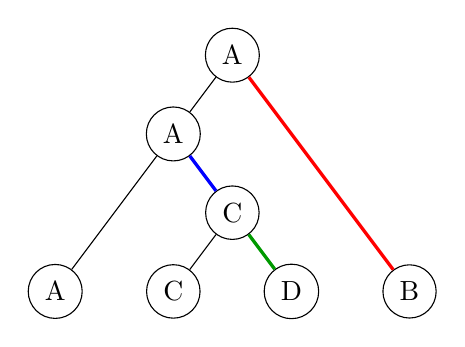
\begin{tikzpicture}
  [every node/.style = {circle, draw}]
  \node (a) at (0, 0) {A};
  \node (c) at (1.5, 0) {C};
  \node (d) at (3, 0) {D};
  \node (b) at (4.5, 0) {B};

  \node (cd) at (2.25, 1) {C};
  \node (acd) at (1.5, 2) {A};
  \node (abcd) at (2.25, 3) {A};

  \draw [red, very thick] (abcd) -- (b);
  \draw (abcd) -- (acd);
  \draw [blue, very thick] (acd) -- (cd);
  \draw (acd) -- (a);
  \draw (cd) -- (c);
  \draw [green!60!black, very thick] (cd) -- (d);
\end{tikzpicture}

\end{document}
